\documentclass[a4paper]{article}
\usepackage[top=2in, bottom=1.5in, left=1in, right=1in]{geometry}
\usepackage{float}
\usepackage{hyperref}
\usepackage{tabularx}
\usepackage{tikz}
\usepackage{caption}
\usepackage{fancyhdr}
\usetikzlibrary{positioning}
\setlength\parindent{0pt}
\setlength{\headheight}{15.2pt}
\setlength{\topmargin}{0pt}
\setlength{\textheight}{630pt}
\pagestyle{fancy}

\title{A Brief Survey of Problems and Solutions \\ in Robotic Swarms}
\author{S.J.A. Bekhoven  \and
    S.P. Metman \and
    M.J. Rogalla}
\date{\today}

\begin{document}
\maketitle

\begin{abstract}
Swarm robotics has become a prominent and promising research area in the recent years. 
It has great potential use for a large variety of applications. 
In order to not forget the big picture, we believe that a survey of a few basic problems in this field should be given. 
This survey presents a concise overview of a few problems that the robotic swarms research area has faced. For each problem we provide a small discussion as to which approaches were chosen. 
Finally we mention the remaining issues for each problem. 
Each of the algorithms can be categorized by their usage of range information and location information. 
We show the problems which come with each of these categories and compare the scalability and performance of each approach. 
This provides insight into the properties of the algorithms which affect the scalability and the performance. 
Addressing these problems and their approaches gives a better overview and offers inspiration to solve other problems.
Finally we give a general conclusion regarding the recent advancements in robotic swarms.
\end{abstract}

% Do not compile individual files, compile only this main file.

\section{Introduction}
  %!TEX root = ../Bachelorseminar-RoboticSwarms.tex

Swarm robotics has become a prominent and promising research area in the recent years. 
It has great potential use for a large variety of applications, some of which have already been successfully implemented. 
We want to provide a global overview of the main problems found in the research area of robotic swarms. 
Many articles already exist which give an overview of applications and used practices in this area, but often do not explain the problems underlying these practices. 
Therefore, we focus on providing a problem-oriented overview of the robotic swarms, while also providing a general overview of best practices and solutions of these problems.\\
\\
We start by defining some terminology, since some of the terms used in robotic swarms are ambiguous and can be interpreted in different ways.
We define a swarm as a scalable network of robots which consists out of more than two robots.
Furthermore, we only consider robotic swarms in which every robot has some form of distributed intelligence.
An exception is of course when a swarm of multiple robots is controlled by one control station.
Because the swarm robots have to communicate either directly or indirectly with each other, the swarm will still have some form of distributed intelligence to function.
% Thus, according to our original definition, we still regard it as a swarm. \\
\\
\\
Robotic swarm algorithms can roughly be characterized by their location type and their information type. Algorithms can then respectively be either \emph{location-based} or \emph{location-free} and either \emph{range-based} or \emph{range-free}:
\begin{description}
	\item[Location-free] Robots have no knowledge and do not keep track of their absolute or relative location.
	%A robotic swarm is \emph{location-free} if the swarm has no knowledge of the boundaries of the location it is in, whether it is provided at the beginning or is actively searched for during the execution of the algorithm. 
	\item[Location-based] Robots have perfect knowledge or keep track of their absolute or relative location.
	%A robotic swarm is \emph{location-based} if each individual robot in the swarm has the knowledge of its absolute or relative location.
	\item[Range-free] Robots do not communicate or communicate via some kind of central base.
	%A robotic swarm is \emph{range-free} if each robot can detect the presence of other nearby robots or obstacles, but does not store or measure the distance towards the other object.
	\item[Range-based] Robots communicate within predetermined range.
	%A robotic swarm is \emph{range-based} if each robot in the swarm keeps track of the exact distance between itself and the other robots in the swarm or obstacles. 
\end{description}

In the following sections, we compare the algorithms by two characteristics. 
The first characteristic is \emph{scalability}, by which we mean the ability of maintaining performance when the population in the robot swarm is increased. 
The second is \emph{performance}, by which we mean the general efficiency. 
We define efficiency separately for each problem before comparing the algorithms of that problem. 
We do this because the solutions have different ways of expressing efficiency for each problem.\\

A composite problem is a problem composed of multiple main problems in such a way that these main problems influence the working of the solutions. 
Although such a composite problem can be singled out, a lot of the main problems have some form of overlap too, although not with significant impact. 
The main problems Dispersion and Source Localization both include the Formation problem, and the Collective Transport is composed of the Formation problem among others.
The Exploration problem is more of an extension to the Dispersion problem. 
This relationship is shown in the Figure~\ref{fig:ProblemsOverview} \\
\begin{figure*}
  \centering
  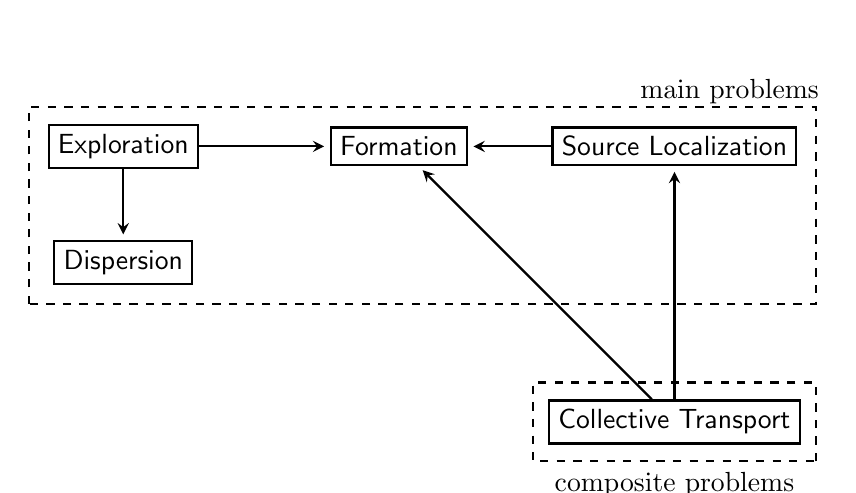
\begin{tikzpicture}[->,>=stealth,shorten >=2pt,auto,node distance=3.5cm,
    thick,main node/.style={fill=white,draw,font=\sffamily}]
    \node at (7.7,0.7) {main problems};
    \node at (7,-4.3) {composite problems};
    \draw[fill=white,dashed] (-1.2,-2) rectangle (8.8,0.5);
    \draw[fill=white,dashed] (8.8,-4) rectangle (5.2,-3);
    \node[main node] (1) {Exploration};
    \node[main node] (2) [below= 0.9cm of 1] {Dispersion};
    \node[main node] (3) [right of=1] {Formation};
    \node[main node] (4) [right of=3] {Source Localization};
    \node[main node] (5) [below of=4] {Collective Transport};

    \path[every node/.style={font=\sffamily\small}]
      (1) edge [right] node[left] {} (2)
      (4) edge [right] node[left] {} (3)
      (5) edge [right] node[left] {} (4)
      (5) edge [right] node[left] {} (3)
      (1) edge [right] node[left] {} (3);
  \end{tikzpicture}
  \caption{Problem Composition Overview} \label{fig:ProblemsOverview}
\end{figure*}



The remainder of this paper is then structured as follows. 
In Section~\ref{sec:Formation} until Section~\ref{sec:Localization} we define the main problems in robotic swarms. 
Then, in Section~\ref{sec:CollectiveTransport}, we discuss the composite problem Collective Transport. 
For each problem we mention the possible real-life applications, their subproblems and the underlying algorithms of the solutions.
After that we discuss the characteristics of each algorithm, the corresponding (dis)advantages and where possible some remaining problems.
For more information on the operation of the mentioned algorithms, you can check the references provided. 
Finally we briefly discuss our observations in Section~\ref{sec:Discussion}.





\section{Formation}
  \label{sec:Formation}
  %!TEX root = ../Bachelorseminar-RoboticSwarms.tex

Formation is the problem of controlling the relative position and orientation of the robots in a group while allowing the group to move as a whole. \cite{consolini2008leader}
Formation is one of the key problems in robotics swarms, as it is a primitive in many other problems and composite-problems.
In particular it is used in the collective transport problem, where a swarm has to hold a formation to move an object. 
An example of such an application is moving an object with robotic cars. \cite{mas2012object}
An application in which formation is also extensively used is area surveillance, where formation is used to increase coverage. \cite{burkle2011towards}
A more specific example is indoor surveillance, where ground robots are already being used. \cite{di2010autonomous, rybski2000team}
\\

Two main subproblems arise from the original formation problem: the \emph{communication problem} and the \emph{formation stability} problem.\\
In the \emph{communication subproblem} the algorithm needs to come with a communication algorithm for usage within the robotic swarm. 
Each of these algorithms differ in these inter-robot communication strategies. 
Some algorithms only rely on local communication while other algorithms communicate via a centralized system.
This affects if an algorithm is range-free or range-based. 
Some algorithms keep track of each robot's location and are thus location-based, while others are location-free.
These locations can be be communicated through different ways of communication. \\

The \emph{formation stability problem} is another subproblem, which each of these algorithms have to deal with.
Specifically, the algorithm should be able to dampen the effects of disturbance propagation. 
This means that when one robot in the formation encounters a disturbance and moves out of formation, how is this situation handled in the swarm. 
The effect of such a disturbance should be reduced.
We call this the \emph{source disturbance dampening} subproblem. 
For each algorithm, we review how these problems are solved.

\subsection{Algorithms}
Many different algorithms have been used to solve the formation problem. \cite{chen2005formation,consolini2008leader}
These algorithms can categorized as: leader-follower algorithm \cite{consolini2008leader,das2002vision}, 
behavior-based algorithm \cite{balch1998behavior,lawton2003decentralized}, 
and virtual structure algorithm \cite{ren2004decentralized,do2007nonlinear}. \\
The algorithms are build upon in later algorithms to create more novel algorithms. A few of these algorithms are: 
virtual space configuration \cite{wee2013formation}, 
fuzzy formation control \cite{ranjbar2012novel},
and team-work software control. \cite{kaminka2013use} 
We compare these algorithms primarily by their performance and their scalability. 
We define \emph{performance} in how quickly the formation can be formed again after the formation is lost (disturbance dampening). 
This can also be referred to as the stability of the formation.
We discuss each of these algorithms separately in the next section and make a comparison at the end of the chapter.

\subsubsection{Leader-follower algorithm}
First, we discuss the leader-follower algorithm. 
In the leader-follower algorithm a robot of the swarm is designed as the leader.
The leader moves along a predefined path while the other robots, the followers, are maintaining a desired distance and orientation to the leader. \cite{consolini2008leader}
This can be implemented by equipping the leader robot with a omni-directional camera and logical sensors, like an obstacle detector and a collision detector.
The leader then instructs the followers through local communication. \cite{das2002vision}
The main problem with this algorithms is that it depends heavily on the leader and when something happens to the leader, the algorithm fails. 
Source disturbance dampening is done by the leader; the leader communicates any disturbances to its followers.

\subsubsection{Behavior-based algorithm}
The second algorithm we discuss is the behavior-based algorithm. 
In the behavior-based algorithm, every robot in the swarm is programmed with a certain behavior. 
These behaviors may differ between robots.
Some examples of these behaviors are the collision-avoidance behavior and the target-seeking behavior. 
The action that is taken is decided by weighing the relative importance of each behavior. \cite{consolini2008leader}
These behaviors can then be used to maintain certain formations like a line, a column, a diamond and a wedge. \cite{balch1998behavior}
The dynamics and stability of this algorithm are calculated with the Lapyunov function, which is used to account for many stability issues. \cite{lawton2003decentralized}
In this algorithm, the decisions are not made locally, but real-time data is sent to a system which then decides what each robot should do based on their behaviors.
Disturbance source dampening is applied by the different behaviors assigned to each swarm robot.

\subsubsection{Virtual structure algorithm}
The last of the more basic algorithms is the virtual structure algorithm. 
The virtual structure algorithm considers the formation as a single virtual rigid structure such that the behavior of the robotic system is similar to that of a physical object. 
Desired trajectories are not assigned to each single robot but to the entire formation as a whole. 
The behavior of the formation in this case is exactly predictable but also generates a  large overhead. \cite{consolini2008leader}
Such a virtual structure is thus decentralized and appropriate distributed control strategies can be made. \cite{ren2004decentralized}
The control system can be structured in four sequential stages: defining the dynamics of the virtual structure, 
translating the motion of the virtual structure into the desired motion for each robot, 
deriving output feedback for each robot,
and introducing formation feedback from each robot to the virtual structure. \cite{do2007nonlinear} 

\subsubsection{Virtual space configuration}
Aside from these three algorithms which have become a standard way for implementing formation control, more novel algorithms have been developed. 
One of these algorithms is the virtual space configuration algorithm. \cite{wee2013formation}
This algorithm uses a leader-follower algorithm, but each robot uses virtual space and virtual robots inside that space.
These virtual robots are then used by each robot to avoid collisions. 
The main difference is then that multiple follower robots in formations can maintain formation without crashing (using only virtual collisions), and they can have scalability of formation. 
This algorithm is range-based and location-free, but produces a lot of overhead in local communication.

\subsubsection{Fuzzy formation control}
Another novel algorithm is fuzzy formation control.\cite{ranjbar2012novel}
In robotic swarms, optimal control techniques have been found to treat robust stabilization and tracking problems. 
But in these cases, the exact model of the system has to be known. 
But this fuzzy formation control technique provides a robust scheme with a fuzzy logic estimator to implement effective controls for uncertain dynamic models.
This way, the exact model does not need to be known, as nonlinearity, external disturbances and model uncertainties are dealt with by fuzzy approximation.

\subsubsection{Teamwork software control}
Lastly, the last formation control we discuss is the teamwork software control. \cite{kaminka2013use}
This algorithm combines different control algorithms and tries to integrate this in one formation control algorithm.
It is mostly behavior-based, and each of the robots in the swarm has its own behavioral process. 
But instead of carrying out its behavior directly, each robot communicates with each other to set a ``team flag''. 
When every robot agrees with this flag, only then is this order carried out. 
This resembles the virtual structure control algorithm a little, as in that the swarm is considered as a whole. 
This algorithm is location-free but range-based, and produces more overhead than the behavior-based algorithm.

All the algorithms try to solve the formation problem. 
%The algorithms are all location-free, due to the fact that they have to work with relative location and not absolute locations. If there is
These algorithms are all location-free, which makes sense.  
Because when an algorithm is location-based, all robots know their exact locations and can adjust their position, and the problem is already solved. \\
The most important attribute for each algorithm is the performance, so how stable the formation is, as in how good the formation can be kept. 
This performance increases in the later algorithms, which expand upon the more basic algorithms. 
But, as the performance increases, the scalability lower for algorithms which communicate via a central framework. 
Take for example the teamwork software control algorithm. 
This algorithm provides high performance, but also creates lots of overhead activity due to its central communication.
This decreases the scalability of this algorithm significantly.\\

\subsection{Discussion}
  \begin{table}[H]
  \renewcommand{\arraystretch}{1.3}
  \label{table_alg_formation}
  \centering
\scalebox{0.85}{
  \begin{tabular}{|l|l|l|l|l|}
    \hline
    \bfseries Algorithm & \bfseries Range & \bfseries Location & \bfseries Performance & \bfseries Scalability\\
    \hline
    Leader-follower & Range-based & Location-Free & Medium & Low\\\hline
    Behavior-based & Range-free & Location-Free & Medium & High\\\hline
    Virtual structure& Range-based& Location-Free & High  & Medium\\\hline
    Virtual space & Range-based& Location-Free & High  & Low\\\hline
    Fuzzy control& Range-free& Location-Free & High  & Medium\\\hline
    Teamwork control& Range-based& Location-Free & High  & Low\\\hline
    \end{tabular}
    }
  \caption{Overview of Formation Algorithms}
  \end{table}

Concluding this chapter we discuss the future problems of these algorithms. 
As can be seen from the algorithms, centralized communication reduces scalability. 
Although centralized communication does provide high performance, the lower scalability is a downside. 
Decentralized algorithms are more likely to be scalable, and is an interesting topic for future solutions to the formation problem.
Another problem faced by these algorithms is reliability, especially for the leader-follower algorithm. 
If the leader is lost (for example destroyed), the algorithm does not work anymore. 
A new leader could be chosen among the followers, but this is not taken into account in all the leader-follower algorithms. 
This is a problem that most of these algorithms do not take in account.  


\section{Dispersion}
  \label{sec:Dispersion}
  %!TEX root = ../../Bachelorseminar-RoboticSwarms.tex
We consider dispersion as one of the key problems needed to be solved in Robotic Swarms.\cite{ugur2007dispersion,mclurkin2007distributed,ludwig2006robotic} Dispersion can be compared to the blanket coverage problem, which is defined by in one of the first papers written on the topic of swarm robots: \emph{Command Control for Many-Robot Systems}.\cite{gage1992command} The objective of blanket coverage is defined as ``achieving a static arrangement of elements that maximizes the detection rate of targets appearing within the coverage area.''\cite{gage1992command} The difference between dispersion and formation is often confused. While formation is trying to maintain explicitly specified spacing relationships, dispersion tries to find the best ``formation'' for the current environment. \\

Due to the fact that dispersion is one of the fundamental problems in robotic swarms, it has a great number of applications.
Some of these applications include, but are not limited to exploration, surveillance, military response, disaster response and planetary exploration.\cite{ludwig2006robotic,Penders2011,mclurkin2007distributed} 

\subsection{Algorithms}
In this section we discuss a few categories of approaches which are used to solve the dispersion problem.
Starting from the simpler algorithms which are based on the approach which includes randomness such as random-walk and wall-following, we show the problems that the dispersion problem has faced in the past and how the newer algorithms have solved these problems.
Further we motivate as to why the algorithms are put into a specific category and discuss the scalability and performance for each type of algorithm.
For more information on the operation of the mentioned algorithms, please consult the references.

  \begin{table}[H]
  \renewcommand{\arraystretch}{1.3}
  \label{table_alg_dispersion}
  \caption{Overview of Common Dispersion Algorithms}
  \centering
    \begin{tabular}{|l|l|l|l|l|l|}
    \hline
    \bfseries Algorithm & \bfseries Approach & \bfseries Range & \bfseries Location & \bfseries Performance & \bfseries Scalability\\
    \hline
    \bfseries Random Walk & Brute-Force & Range-Based & Location-Free & Medium & High\\\hline
    \bfseries Follow Wall & Brute-Force & Range-Based & Location-Free & Low & Low\\\hline
    \bfseries Directed Dispersion & Inverse-Vector & Range-Based & Location-Free & Medium & High\\\hline
    \bfseries Seek Open & Inverse-Vector & Range-Based & Location-Free & Low & Medium\\\hline
    \bfseries Fiducial & Inverse-Vector & Range-Based & Location-Free & Medium & High\\\hline
    \bfseries DFLF & Graph-Theory & Range-Based & Location-Based & Medium-High & Low\\\hline
    \bfseries BFLF & Graph-Theory & Range-Based & Location-Based & High & Low\\\hline
    \bfseries Clique-Intensity & Graph-Theory & Range-Based & Location-Free & Medium & High\\\hline
    \end{tabular}
  \end{table}

\subsubsection{Randomness Approach}
%TODO: Find a few more references talking about random walk and follow-wall concerning usage in Robotic Swarms
The algorithms in this category try to solve the dispersion problem with an approach which relies on randomness to perform the dispersion.
All of these algorithms are mainly location-free, but often include collision detection which makes them range-based.\\
The most pre-eminent algorithm in this category is the \emph{Random-Walk} algorithm due to its simplistic nature and efficiency. 
The \emph{Random-Walk} algorithm changes the robot's orientation randomly and moves it forward until an obstacle is detected. The algorithm then repeats the steps indefinetely.\cite{morlok2007dispersing}
The algorithm is very scalable, due to the simple set of steps that have to be performed and due to its non-interdependence of other robots in the swarm.
A minor drawback with the \emph{Random-Walk} algorithm is that it does not guarantee uniform dispersion.
Due to the reliance on randomness, the algorithm is not optimal. If low-energy consumption has a high priority in the system, we do not recommend the usage of this algorithm.
In all other situations which allow its usage the \emph{Random-Walk} algorithm is greatly recommended due to its satisfying performance and highly rated scalability.\\
Another algorithm which is also used for dispersion purposes is the \emph{Follow-Wall} algorithm.\cite{morlok2007dispersing}
Originally the algorithm is not random, but follows an exact set of rules depending on the environment. 
The algorithm is created for a non-dynamic environment and not for usage in robotic swarms.
The robot is unable to see the difference between robots and other obstacles. This creates the possibility for robots to constantly follow each other, while thinking that they're actually moving around a wall or other static obstacly.
The performance rating is low due to the meager amount of randomness and its unability to gurantee the uniformity of the dispersion. The scalability is also rated low, due to the performance deterioration when increasing the scale.\\


\subsubsection{Graph Theory Approach}
The algorithms which are inspired by graph theory can be divided into two sub-categories: algorithms inspired by tree search algorithms and algorithms inspired by connectivity in graphs.\\

In a paper on algorithms for rapidly dispersing robot swarms in unkown environments\cite{hsiang2004algorithms}, two tree search inspired algorithms were named.
The paper mentions two strategies: \emph{Depth-First Leader-Follower(DFLF)} Strategy and the \emph{Breadth-First Leader-Follower} Strategy.
The implementation of these algorithms are mainly considered as \emph{location-based} algorithms, due to the fact that they work with grids which require absolute or relative positioning.
The \emph{BFLF} algorithm, requires the robots to travel less compared to the \emph{DFLF} algortihm. The DFLF algorithm is furthermore also more computationally expensive than the DFLF algorithm.
Further, there are no big differences during the execution of both algorithms, and thus BFLF has the preference.
Due to the high amount of computation which needs to be done centrally, the scalibility of this type of algorithms are rather low.
Every robot has to be taken care of by one or multiple robots. By centralizing this computation, there is a greater risk of failure due to instability compared to decentralized control.\\

The problems that these types of algorithms face are not theoretical, but are coming forth from the category that they are in. They are all location-based. Often it is impossible to know the exact location, even if it's relative, but this a part of the Localization problem, which has to be solved.

One of the algorithms regarding connectivity in graphs is the clique-intensity algorithm.\cite{ugur2007dispersion}
The Clique-Intensity algorithm is range-based since it measures and uses the distance between itself and other surrounding swarm-bots.
The performance and scalability of the algortihm is very high, due to decentralized control.

The Clique-Intensity algorithm faces problems due to the fact that there are high amounts of noise in the wireless intensity signals when used in real-world applications. 
This causes lots of uncertainty in some real world applications.
The work in this area has mostly been theoretical, real-world application is very different compared to theoretical situations.
The Focus should be put on the localization using wireless signals.\\

\subsubsection{Inverse-Vector Approach}
Some examples of the Inverse-Vector approach are the seek-open algorithm\cite{morlok2007dispersing}, the Fiducial algorithm\cite{morlok2007dispersing} and the Uniform Directed Dispersion(UDD) algorithm\cite{mclurkin2007distributed}.
Each of the algorithms basically sense where obstacles and other swarm-bots are relatively positioned and calculate a vector of that data. Afterwards they calculate the inverse of that vector and moves into that direction.
The \emph{Fiducial} algorithm has a advantage over the \emph{Seek-Open} algorithm: it uses a beacon like system, which prevents robots from running into each other and encourages uniformatiy of the distribution.
The seek-open and UDD algorithm use other distance measures mostly using ultrasonic sensors. In both cases the algorithm is a range-based algorithm, where every robot is able to get the relative location. 

It is important to stress that the algorithms should perform periodic checks to detect dynamic changes in the environment, such as other moving robots.


\subsection{Discussion}
The remaining problems in dispersion algorithms can be generally categorized into range-based problems and location-based problems.
All the algorithms that are in these categories are facing similar problems.
The focus needed for the range-based approach needs to be on the uniformity of the dispersion. So how can we guarantee uniformity when dispersing the robots.
In the location-based approach category focus needs to be put on the applicability for real-world applications.
There are minor to no problems in theory, however to actually bring the relative positioning into a grid is quite difficult.
Research in this area should be focussed on creating high-accuracy relative positioning grids.


\section{Exploration}
  \label{sec:Exploration}
  %!TEX root = ../Bachelorseminar-RoboticSwarms.tex

Exploration is a technique in which a swarm of robots tries to fully explore an environment, which is one of the fundamental problems faced in mobile robotics. 
The main goal is to minimize the overall exploration time while still exploring the whole environment. 
The main problem faced when trying to achieve this goal is finding appropriate target points for each individual robot so that they simultaneously explore different regions of the environment. \cite{burgard2005coordinated} \\
Exploration is found in many robotic swarms problems, for example in \emph{path-finding}, \emph{collective transport} and \emph{surveillance}.
Practical applications that use exploration are for example rescue missions. \cite{Naghsh2008,Penders2011}
In this particular paper, a robotic swarm applying exploration is used to assist navigation for firefighters.
It is used in situations in which their vision is blocked by smoke and obstacles. 
A last example of an application is cleaning. \cite{wagner2008cooperative}
Here, exploration is used to clean a surface with cleaning robots as fast and as efficient as possible. 
Exploration is used in many more different robotic swarm applications and is a building block for many other problems.

%OLD
%Exploring an environment is one of the fundamental problems faced in mobile robotics. 
%The main goal is to minimize the overall exploration time and the main problem faced when trying to achieve this goal is finding appropriate target points for each individual robot so that they simultaneously explore different regions of the area \cite{burgard2005coordinated}. 
%Robotic swarm exploration can be used for real-world applications like rescue missions \cite{Naghsh2008,Penders2011}, surveillance \cite{Burkle2010} and cleaning \cite{wagner2008cooperative}.

%!TEX root = ../../main.tex

\subsection{Algorithms}

	\subsubsection{Frontier-based}
	Frontier-based exploration is inspired by the question "Given what you know about the world, where should you move to gain as much new information as possible?". In the orignal implementation by Yamauchi et al. \cite{yamauchi1998frontier} an evidence grid is used in which the occupancy probability is stored for each cell, so it is purely \emph{location-based}.
	All cells are initiated at a certain prior value.
	In the further process they are divided in three classes according to their value: open, unkown or occupied.
	Every open cell adjacent to an unkown cell is labeled as a frontier edge cell.
	Every group of frontier cells above a minimum size is considered a frontier.
	Once these frontiers have been deteced, the robot navigates to the nearest unvisited frontier.
	While travelling already found obstructions can be avoided.
	When the robot reaches its destination it does a 360 degree sensor sweep and adds the new information to the evidence grid.
	When the robot doesn't make progress for a certain amount of time it will conclude its current location is inaccessible and update its evidence grid.
	Whenever a robot arrives at a new frontier it creates a local grid, which is shared with all other robots.\\
	\\
	A limitation of this approach is that since navigation is independent, robots may waste time navigation to the same frontier.
	This will either cause an avoidance manoeuvre or the robots will block each other.
	In the last case the robots will mark their destination frontiers as inaccessible.


	% http://www4.cs.umanitoba.ca/~jacky/Robotics/Papers/frontierExploration.pdf

	\subsubsection{Frontier-based with bidding}
	The implementation discussed in a paper by Sheng et al. \cite{sheng2006distributed} is an extended form of the frontier-based algorithm.
	It is extended with a bidding algorithm which solves the problem of robots heading for the same frontier or robots blocking each other as described above.
	Furthermore the robots have limited range and this approach therefore not only is \emph{location-based}, but also \emph{range-based}.
	In this implementation all robots start from initital positions which are very close to each other.
	The robots broadcast their bid to all other robots in the sensor range and wait for a constant time.
	If their bid is the best, they travel to the frontier-based best location to go to.
	If not they remap, recalculate and bid again.
	The bid exists of information about each cell (based on the current map and the targets of robots in the neighbourhood), the distance to each cell (based on Dijkstra) and a nearness measure (to sustain communication between robots).
	By implementing the nearness measure, the robots tend to stay close to each other. 
	This results in better communication, which leads to less repeated coverage and less exploration time in comparison to general frontier-based approaches.
	Furthermore we see that when increasing the range the exploration time and the traveled distance dramatically decrease.	

	% http://ac.els-cdn.com/S092188900600114X/1-s2.0-S092188900600114X-main.pdf?_tid=33bf4874-ab01-11e3-a577-00000aacb35f&acdnat=1394750920_0424c8c4f3098477e3985d83f4f339f2

	\subsubsection{Market-economy based}
	Zlot et al. have chosen another approach which also uses some kind of bidding principle called a market architecture. \cite{zlot2002multi}
	The robots have perfect knowledge of their location and keep track of a map.
	Furthermore the robots communicate with each other over limited range, so this is an \emph{location-based} and \emph{range-based} approach.
	The distributed algorithm starts by generating a list of goal points.
	Goal points are generated to navigate to with three different strategies.
	The strategies used by the robots may be all the same, vary across robots or even over time.
	The three strategies are 1) random, 2) greedy exploration and 3) space division by quadtree.
	All strategies are very simplistic, because the intention is that the market architecture removes the inefficiencies.
	The goal points generated are greedily ordered (shortest-path).
	The robot then tries to sell all of its tasks to robots it can communicate with by auction for a specified amount of time.
	Each goal point is awarded a certain revenue according to the amount of information it will provide and a certain cost according to the resources it will cost to achieve it.
	The robots start bidding and the highest bidder is awarded the task if it is higher than the minimum amount set by the auctioneer.
	After trying to sell all of its tasks by auction the robot travels towards a goal point.
	If it reaches the goal point, it generates a certain amount of new goal points, starts off with its next goal and offers its remaining goals to other robots.
	Finally at regular intervals robots can exchange pieces of their own map with each other for a certain cost/revenue depending on the expected utility.
	When asked, all robots send their maps to a central base, so a global map can be created.\\
	\\
	Surprisingly simulation shows that when only using the random strategy the algorithm performs just as good as when using the quadtree strategy.
	Furthermore the algorithm using the random or quadtree strategy is compared to a communicationless situation.
	We can see that allowing the robots to communicate via the market place architecture improves the exploration efficiency with a factor of $3.4$ in a four-robot system.
	The system could be improved by for example using a time-based cost scale instead of a distance-based for minimizing while exploring.

\begin{table}[H]
	\renewcommand{\arraystretch}{1.3}
	\caption{Overview of Common Localization Algorithms}
	\label{table_alg_exploration}
	\centering

    \begin{tabular}{|l|l|l|l|l|l|}
	    \hline
	    \bfseries Algorithm & \bfseries Range-type & \bfseries Location-type & \bfseries Performance & \bfseries Scalability\\
	    \hline
	    \bfseries Frontier-based & - & Location-based & Medium & Low\\
	    \hline
	    \bfseries Frontier-based with bidding & Range-based & Location-based & High & High\\
	    \hline
	    \bfseries Market Economy based & Range-based & Location-based & Medium-high & Medium\\
	    \hline
    \end{tabular}
\end{table}



%Coordinated multi-robot exploration
% http://ieeexplore.ieee.org/stamp/stamp.jsp?tp=&arnumber=1435481
%\cite{burgard2005coordinated}

%Collaborative multi-robot exploration
% http://www.cs.cmu.edu/afs/.cs.cmu.edu/Web/People/motionplanning/papers/sbp_papers/integrated2/burgard_multi_robot_explor.pdf
%\cite{burgard2000collaborative}

%Coordination for Multi-Robot Exploration and Mapping
% http://isl.ecst.csuchico.edu/DOCS/Papers/simmons2000coordination4MultirobotExploration.pdf
%\cite{simmons2000coordination}

%Multi-robot exploration Controlled by a Market Economy\\
%Market-place algorithm, seems good, ++
% http://repository.cmu.edu/cgi/viewcontent.cgi?article=1174&context=robotics&sei-redir=1&referer=http%3A%2F%2Fscholar.google.nl%2Fscholar%3Fq%3Dmulti-robot%2Bexploration%26btnG%3D%26hl%3Dnl%26as_sdt%3D0%252C5#search=%22multi-robot%20exploration%22
%\cite{zlot2002multi}

%Multi-robot exploration under the constraints of wireless networking
%http://ac.els-cdn.com/S0967066106001547/1-s2.0-S0967066106001547-main.pdf?_tid=2dbdf35e-ab00-11e3-b5b9-00000aab0f6c&acdnat=1394750480_8d4547f2c72259f166f10342891ca745
%\cite{rooker2007multi}

%A practical, decision-theoretic approach to multi-robot mapping and exploration
% http://ieeexplore.ieee.org/stamp/stamp.jsp?tp=&arnumber=1249654
%\cite{ko2003practical}

%Multi-robot collaboration for robust exploration
%\cite{rekleitis2001multi}
% http://download.springer.com/static/pdf/926/art%253A10.1023%252FA%253A1016636024246.pdf?auth66=1394923400_27944ba6f349eb21a47a2c60f843ab9f&ext=.pdf

%Distributed multi-robot coordination in area exploration +++++
%\cite{sheng2006distributed}
% http://ac.els-cdn.com/S092188900600114X/1-s2.0-S092188900600114X-main.pdf?_tid=33bf4874-ab01-11e3-a577-00000aacb35f&acdnat=1394750920_0424c8c4f3098477e3985d83f4f339f2

%Coverage for robotics–A survey of recent results

%multi-robot coverage??

\section{Source Localization}
  \label{sec:Localization}
  %!TEX root = ../Bachelorseminar-RoboticSwarms.tex

\subsection{Applications}
Source localization is a technique in which a swarm of robots try to locate a specific point, often used to find sources of disturbance. 
The main goal of this technique is to find all sources of disturbance as fast as possible. 
Source localization is used in virtually any other robotic swarms technique, because in most techniques something has to be found, whether it is a source or an object. \\

Obviously, this means that this technique has many practical applications.
A few of these examples will be mentioned here. 
A first example is chemical plume tracing, in which localization is used to detect clouds of high density chemicals. \cite{zarzhitsky2005distributed}
Another example which looks a lot like chemical plume tracing, is radiation source search. \cite{bashyal2008human} The difference is that in this case the source of leaking radiation is searched for, and not only for high density clouds. 
A third example is searching for fire, used to assist fire-fighters in their every-day work. \cite{marjovi2009multi}
As can be seen, this technique can be used to look for all kinds of emission sources, if the robots have the right sensors installed. \cite{cui2004swarm}
Although many practical applications can be found, a large amount of the work done in this field is purely theoretical.
This is due to the fact that the price of these individual robots is still rather high and thus it is expensive to produce a swarm.


%Source localization is used in a large category of robotic-swarm applications. 
%Some of the topics include, but are not limited to: chemical plume tracing\cite{zarzhitsky2005distributed}, radiation source search\cite{bashyal2008human}, fire searching\cite{marjovi2009multi} and other types of emission source localization\cite{cui2004swarm}. %A large amount of the work done in this field is purely theoretical, this is due to the fact that the price of these individual robots is still rather high and thus it is expensive to produce a large quantity.
%The main techniques underlying these applications include: control, communication, path-planning and distribution.\cite{Li2012}

%!TEX root = ../../main.tex

\subsection{Algorithms}
Localization of targets with robotic swarms is an area which has been receiving a lot of research attention in the past few years. 
The main goal is to design an algorithm that effectively allows a swarm of robots to explore an unknown area and find the target(s).
Localization as discussed here basically exists of two parts: exploring and searching.
In this chapter mostly only the latter, so the actual localization, is discussed.
For exploration methods the the chapters about \emph{exploration} and/or \emph{dispersion} should be read.

	\subsubsection{Gradient-based}
		% http://ac.els-cdn.com/S1574119208000618/1-s2.0-S1574119208000618-main.pdf?_tid=fcc68570-aaed-11e3-bbdc-00000aacb360&acdnat=1394742667_d3fd3d62038328cd6bea316cff88955e
		In \cite{zhang2009gradient} a centralized implementation of a gradient-based algorithm is discussed in which all robots have knowledge of their location.
		Each robot uses a received signal strength indicator to predict the location of the target with a certain probability and reports back to the base.
		The base collects all readings and plans to create a global map and an uncertainty area which is sent to all robots.
		With this data the robots continiously predict the target position with increasing accuracy as they move towards the target.
		In general hill climbing or gradient-based algorithms are limited to single-source searches.
		The proposed algorithm in this paper leads to a 40\% reduction in time compared to random path models and in \cite{dhariwal2004bacterium} we see it performs approximately twice as good as a biased random walk, which is discussed later.

	\subsubsection{Particle Swarm Optimization}
		In Particle Swarm Optimization (PSO) a number of particles is randomly distributed over an unkown space of a problem or function. 
		Each particle evalues its current location according to a certain fitness function and then calculates the best position to go to according to its own historical best position and the historical best positions of the particle(s) in its neighbourhood.
		To prevent the particles from agglomeration a certain randomness is often implemented. 
		By continuously looking for a better position by helping each other, the swarm of particles eventually positions itself at the position of target. \cite{poli2007particle}\\
		\\
		A model of a PSO inspired algorithm in which every robot has perfect knowledge of its location and can communicate and sense other robots within a certain range can be found in \cite{pugh2007inspiring}.
		To model robotic swarm search a couple of modifications had to be made, for example: changing PSO's discrete time to continuous time, handling the movement limitations and collisions of robots and limiting the particle neighbourhood (range) of each robot, which is unlimited in general PSO.
		With the model the effect of the communication range and the number of robots have been investigated.
		Main results are that the algorithm indeed achieved better results (smaller final distance to source) when enlarging the number of robots.
		Furthermore the detection of the source with small communiation achieved poor results, but improved dramatically as the range increased.
		At the maximum range the average final distance to the target was the smallest compared to all other communication ranges.\\
		\\
		In \cite{derr2009multi} a decentralized application of PSO is implemented.
		The developed algorithm is \emph{location-free} and \emph{range-based}.
		The targets are equipped with a cell phone that radiates a radio frequency signal that can be detected by the robot, which can wirelessly communicate with limited range.
		The paper shows that a distributed algorithm based on PSO can easily overshoot targets, but that this can be prevented with a correction on the standard PSO formula.
		Furthermore it concludes by experiments that the variation in received signal strenghts (RSS) in an indoor environment significantly increases the robot search time in finding a target.

	\subsubsection{Glowworm Swarm Optimization}
		In Glowworm Swarm Optimization (GSO) the idea is to distribute "glowworms" randomly over the area and let them, according to the fitness function, carry a certain lumeniscence quantity called luciferin. 
		The closer they get to the target the more luciferin they contain - thus the brighter they are - and the more they attract other glowworms. 
		In every movement step each glowworm moves towards a neighbour within a certain range that carries more luciferin, so they eventually conglomerate at the target. 
		The glowworms have a communication range that varies at each step with a certain randomness, to make sure not all agents focus on the same target. \cite{krishnanand2006glowworm}\\
		\\
		A robotic implementation based on GSO is succesfully ipmlemented and described in \cite{krishnanand2005detection}.
		In comparison to PSO based algorithms this algorithm is completely \emph{memoryless}.
		It is shown that the number of targets captured by the algorithm is a strong function of the sensor range.
		Therefore, because we do not know how many targets to capture in an unkown environment, the sensor range is made a varying parameter.
		Besides it shows that when blocking regions the inter-agent communication helps to still let robots select a feasible direction towards the source.

	\subsubsection{Biasing Expansion Swarm Approach}
		An implementation of the Biasing Expansion Swarm Approach (BESA) is discussed in \cite{cui2004swarm}.
		In this approach robots have communication possibilities over limited range and together create a ad-hoc wireless network for global communication capibility.
		Each agent maintains an occupancy grid map to represent the environment wchich is initiated with all cells unexplored.
		After deployment robots share their locations and sensed concentrations with the swarm.
		To uphold seperation a robot does not enter a cell which is already occupied and maintains cohesion by using a gradual expansion algorithm.
		Robotos can therefore only move to cells that are unexplored, unoccupied and next to another robot in the swarm: the expansion cells.
		To make sure the swarm moves to the emission source, each expansion cell is given a certain biasing parameter, based on the number of agents, the distance between the expansion cell and the robot and the concentration sensed at the particular cell.
		The robot will choose the expansion cell with the highest parameter, so that the swarm will eventually move to the direction of the higher concentrations.
		The BESA algorithm developed in this paper performs twice times better than the general gradient-based approaches.

	\subsubsection{Biased Random Walk}
		A rather simple algorithm inspired by nature is the Biased Random Walk (BSR) described in \cite{dhariwal2004bacterium} approach inspired by bacteria. 
		Implementations of this algorithm do not use communication or any form of localization. 
		Robots only have the possibility to perform two actions: move or tumble. 
		When tumbling the robot just turns into a new random direction. 
		When moving the robot travels a certain distance into the chosen direction. 
		If the robot senses some form of emission, the tumble frequency is lowered, so the distance to be moved increases.

	\begin{table}[H]
  \renewcommand{\arraystretch}{1.3}
  \caption{Overview of Common Localization Algorithms}
  \label{table_alg_localization}
  \centering
    \begin{tabular}{|l|l|l|l|l|l|}
    \hline
    \bfseries Algorithm & Range-type & Location-type & Performance & Scalability\\
    \hline
    \bfseries PSO & Range-based & Location-based/-free & High & High\\
    \hline
    \bfseries GSO & Range-based & Location-free & High & High\\
    \hline
    \bfseries BESA & Range-based & Location-free & Medium & Medium\\
    \hline
    \bfseries Gradient-based & - & Location-based & Medium & Low\\
    \hline
    \bfseries BRW & - & Location-free & Low & High\\
    \hline
    \end{tabular}
  \end{table}

	\subsubsection{Problems}
	The main problem of localization using swarms is (in the case of for example BESA, PSO and GSO) the way robots should cooperate and learn from each other. In other words: how big should the neighbourhood be in which robots cooperate to find targets? One might think it is ideal to use information of \emph{all} robots, but in case of multiple targets, the best position of all robots can be misleading and can cause premature convergence. Therefore in PSO often a particle neighbourhood within a certain range or a constant maximum value of neighbours is chosen and in GSO a range varying each step is being used to make sure multiple targets can be found, while in BESA based approaches the robots create an ad-hoc network to create global communication. In BRW inspired approaches no communication is used at all, which results in low performance compared to all other algorithms.

	\subsubsection{Remaining problems}
	There are a lot of factors that affect the performance of localization of multiple targets, for example the complexity of the implemented algorithms, the number of robots used or the number of targets that is being searched for. As is mentioned in \cite{mcgill2011robot} however there is a lack of validation cases and reference algorithms that form a ground truth for comparative analysis. Therefore it is relatively difficult to compare the developed algorithms for multi-robot localization. Another question in multi-robot localization is which mechanism is to be used after a target has been found. Some papers propose to collect the target and search further, but this is not always possible.

\section{Collective Transport}
  \label{sec:CollectiveTransport}
  %!TEX root = ../../Bachelorseminar-RoboticSwarms.tex

Collective transport of objects is the problem in which a swarm of robots locates a payload and collectively moves the payload to another place, like a homebase. 
This can be compared to the foraging problem; although this implies that a path is made to a certain place, which is not the case in the collective transport problem. \cite{hoff2010two}  
The localization problem is an important part of the collective transport problem and has much overlap .\\
Transporting objects by robotic swarms has many potential applications in many settings, from agriculture to construction to disaster relief. 
Especially in dangerous settings like warzones or radio-active areas, robotic swarms can be a powerful tool to safely retrieve many objects. 
For example, recently Amazon, a large online retailer, announced it would make use of unmanned flying robots to deliver parcels at everyone's door. (www.amazon.com/b?node=8037720011) \\

Collective transport can be seperated into two sub-problems:
\begin{itemize}
	\item  providing safe and reliable transport
	\item moving a payload to its destination.
\end{itemize}
These two different problems will be handled separately because these are two entirely different problems that together compose the whole collective transport problem. 

In algorithms in which swarms are completely autonomous, the focus is on finding the payload and transporting it to its destination.
If a homogeneous swarm is controlled by a single ground station, the algorithm is not considered with finding a payload, but is instead focused on safe, accurate and scalable transport. 
So, we can categorize these problems as user-controlled transportation and autonomous transportation.
In user-controlled transportation, the location the swarm operates in is known, so the algorithms used are location-based.
In autonomous transportation, the location is not know and the algorithms are location-free. \\

\subsubsection{User-controlled swarm transportation algorithms}
A robot, especially a flying robot, can only carry a certain weight, which poses a problem. 
But with a robotic swarm of robots it is possible to transport larger weights in a scalable system, adding swarm robots until you can carry the desired weight. 
So, a swarm of robots is useful for transporting large and/or heavy objects. 
There are two different properties important for user-controlled swarm transportations: safety and scalability. 
To ensure safe and stable transport, swarm robots have to be coordinated in such a way that the payload can be manipulated to a desired position and orientation.
An algorithm for such transport is given in the paper Cooperative manipulation and transportation with aerial robots. \cite{Michael2011}, which we will call the \emph{Aerial Equilibrium} algorithm. 
In this paper, a scalable solution for aerial transport is presented by attaching cables from quadrocopters to the payload, and letting each robot calculate its own movement by a mathematical model. 
This paper formulates general conditions for the payload equilibrium but can be scaled to many swarm robots. 
The mathematical model that is defined in the paper is tested with three quadrocopters and offers a stable transportation for objects, with a degree of freedom related to the amount of robots used and can thus be implemented in the field.
Because the swarm robots do not calculate the exact distance between them, this algorithm can be defined as a range-free algorithm. \\

A second algorithm, used for transporting large objects on the ground, in the water and in the air, considers a multi-robot formation control framework, necessary to coordinate the motions of the robots in the group. 
It is mentioned in the paper payload Manipulation Using Cooperative Mobile Multi-Robot Systems, \cite{Mas2012}, and we will call the algorithm the \emph{Cluster Space Control} algorithm.
This is because control approach used is called cluster space control, and is utilized to control swarm of four four-wheeled robots. 
A user using this type of transportation uses a joystick to input user controls to the whole swarm, after which the control framework specifies the formation and the position and shape of the swarm.
Because the framework calculates the exact range between each robot in the swarm, this algorithm is range-based. 
This control framework allows the user to effectively transport large objects with a scalable set of robots. \\

These two algorithms solve the same problem, namely the problem of transporting large and/or heavy objects, in two entirely different ways. 
The properties are summarized in the following table. 


  \begin{table}[H]
  \renewcommand{\arraystretch}{1.3}
  \caption{User-controlled swarm transportation algorithms}
  \label{table_alg_coltrans1}
  \centering
  \begin{tabular}{|p{3cm}|l|l|l|l|}
    \hline
    \bfseries Algorithm & \bfseries Range &\bfseries Location &  \bfseries Performance & \bfseries Scalability\\
    \hline
     Aerial Equilibrium & Range-free & Location-free & Medium & Low\\\hline
     Cluster Space Control & Range-based & Location-based & Medium & Medium\\\hline

    \end{tabular}
  \end{table}

The main differences between these two algorithms is that in the first mathematical model that is used, each swarm robot individually calculates its position to the other robots and the payload, and is calculating the resulting tension on the payload. 
This way, the rotation and position can be controlled by the position and tension of each robot. 
With the second algorithm, that uses the cluster \emph{cluster space control}, the calculations are not done individually. 
Instead, the framework calculates the position of each robot and the orientation of the payload. 
Thus, these methods both provide stability to the transported payload but in two completely different ways. \\

The problems these algorithms have are that the robots should be coordinated to rely on the location of other robots.
With the mathematical model these are calculated through the tension of the cable attached to each robot, but in the framework it is calculated centrally. 
Problems that are not treated in these articles is how these swarms can locate a payload and autonomously can deliver it to a location. 
Another problem for which no solution is provided is that when these swarms grow to account for heavier objects, the robots will get in each other's way. 
Especially considering transportation, a technique in which every robot must latch on to a payload, this can be hard to practically scale. 

\subsubsection{Autonomous swarm transportation algorithms}
The second sub-poroblem that has to be solved is finding the payload and transporting it to its destination.
This sub-problem can again be divided in four smaller problems:

\begin{itemize}
	\item finding the payload
	\item grabbing the payload
	\item finding target location
	\item moving the payload to the location
\end{itemize}

By defining these sub-problems, the problem is easier to solve and easier to explain each algorithm. \\

Collective transport is the problem in which only one payload has to be moved; we do not concern ourselves with foraging algorithms, which try to find a path to the target to collect multiple objects.
The first algorithm is simple; find the location of the payload through a flocking algorithm and let the swarm robots push the payload to the goal location. 
This algorithm is explained in the paper Collective Transport of Complex Objects by Simple Robots: Theory and Experiments, \cite{Rubenstein2013}, and is called the \emph{flocking} algorithm.
The algorithm is quite simple; every robot looks if it can see the payload location. If so, move towards the location. If not, the robot compares its own heading with the other robots nearby and corrects it until the robot finds the payload location.
Each robot uses one of two behaviors.
 A robot that can see the goals aligns itself towards the goal while moving forward.
 A robot that cannot see the goal uses its IR sensors to determine the heading difference between itself and its neighbors.
 In this paper, the payload location and the goal location are found with light sensors, communicates headings with infrared sensors and uses bump sensors to avoid obstacles. 
The robot latches on to the payload with a velcro strip.
After finding the payload, the robot pushes from an arbitrary side, calculating the amount of force needed in relation to the middle point of mass with its bump sensors and transporting it to the goal location with its light sensor.  
And because the robots latch onto an arbitrary side, scaling of the swarm is extremely effective. \\ 

Another widely used algorithm for transporting objects is the \emph{pheromone} algorithm. 
This algorithms relies on leaving a trail of marks that help guide other swarm robots. 
Although this is algorithm can be used for foraging, it can also be used for retrieving a single payload leading many robots to transport a single payload.
This algorithm is used in the paper Cooperative Transportation by Swarm Robots Using Pheromone Communication. \cite{Fujisawa2013}
 In this paper, this algorithm is tested with swarm-bots which can release and detect spots of ethanol left on the ground, indicating a spot they have to follow. Although the pheromone algorithm implies that pheromones should be used, different varieties of markings can be used, including wireless sensor beacons, drops of paint and even objects. This algorithm is particularly useful for guiding many robots to a payload, if for example the payload is very heavy or if many robots are needed for accurate and/or stable transportation. This algorithm is range-based; it calculates the exact distance to a trail. This algorithm is difficult to implement in dynamic environments, as made marks can dissapear. \\

In looking for swarm algorithms, you want the robots to be as simple as possible. An algorithm that only uses very simple robots is an algorithm that is based on granular convection, als known as the Brazil Nut Effect. This novel method is described in the paper Granular convection to transportation.\cite{Sugawara2012} The algorithms described in this paper are either intended for:

\begin{itemize}
  \item A swarm with homogeneous robots, with no explicit communication
  \item A swarm of heterogeneous robots, composed of robots that change their direction with two different probabilities
  \item A swarm of heterogeneous robots that uses local communication to adjust the fraction of robots that change their direction with higher probability
\end{itemize}

These algorithms listed above are ranked in effectiveness, in which the last one obviously is the most effective, but keep in mind that the robots used to implement this are harder to produce than for the first. \\ The way this algorithm works is as follows. The goal of the swarm robots is to transport the objedct to the goal location. Each swarm robot vibrates with a random force. The goal location outputs a repulsive force. As the robots are randomly placed around the payload and the goal location, the payload gets kicked around by the vibrating swarm robots, until the payload is kicked to the target location. When the swarm increases, the amount of time it costs to transport the payload significantly decreases. With heterogenuous robots, there is more communication between robots to lower the density of the robots around the payload, because slows the process of moving the payload.  This algorithm has different implementations, but is mostly location-free and  range-free. 

A short summarization of these algorithms will be given in the form of this table. 

  \begin{table}[H]
  \renewcommand{\arraystretch}{1.3}
  \label{table_alg_coltrans2}
  \caption{Overview of Collective Transport Algorithms}
  \centering
  \begin{tabular}{|p{5cm}|l|l|l|l|}
    \hline
    \bfseries Algorithm & \bfseries Range & Location & \bfseries Performance & \bfseries Scalability\\
    \hline
    \bfseries Flocking & Range-free & Location-Free & High & High\\\hline
    \bfseries Pheromone & Range-based & Location-Free & Medium & Medium\\\hline
    \bfseries Homogeneous granular\newline convection & Range-free& Location-Free & Low  & High\\\hline
    \bfseries Heterogeneous granular\newline convection & Range-free& Location-Free & Medium & High\\\hline
    \bfseries Heterogeneous granular\newline convection with local\newline communication & Range-based& Location-Free & High & High\\\hline

    \end{tabular}
  \end{table}

These three algorithms are very different from each other, but they all serve a common goal. A problem these algorithms ran into was how to locate the payload, how to move the payload and how to find and reach the goal location. The main problem is locating the payload, something which the granular convection algorithm actually never does.  What these three algorithms have in common is that the transportation process speeds up significantly when adding more swarm robots, but reaches a cap when it becomes ineffective due to maximal density. For this reason, small, easy and cheap to produce swarm robots should be required. The granular convection algorithm has the cheapest robots, but is not necessarily the best, because when the robots become slightly larger and more complicated, more sophisticated and faster algorithms could work. \\

In the mentioned algorithms, moving the payload is mostly done by pushing. In real-life applications this would not always be a good option and a more sophisticated method of attaching should be used. When considering search-and-rescue operations for example, a solution to effectively grab the person to be rescued should be thought of. This is a problem that is yet to be identified in these algorithms and poses a good question for the future.




\section{Discussion}
  \label{sec:Discussion}
  %!TEX root = ../Bachelorseminar-RoboticSwarms.tex

NOTES

- scalability, global communication, 
- lots of overlap

WHAT WE MISS
- mapping
- foraging
- target localization?
- robot localization

In the past sections, we reviewed the most common problems found in the field of robotic swarms. 
These problems however, do overlap, because the problems found in this field often consist of multiple different problems. 
We focused on each problem, highlighting the communication methods of every solution and properties of these communication methods. 
These properties can be summarized in a Venn diagram, allowing for a compact overview of these solutions. 

	\begin{figure}[!ht]
		\label{venn_diagram}

		\centering

		\def\loclb{(180:2.0cm) circle (2.0cm)}
	  	\def\loclf{(0:2.0cm) circle (2.0cm)}
	  	\def\locrb{(90:2.0cm) circle (2.0cm)}
	  	\def\locrf{(270:2.0cm) circle (2.0cm)}

	    \begin{tikzpicture}
			% standard figures
			\draw \loclb node [text=black] {Location-based};
			\draw \loclf node [text=black] {Location-free};
			\draw \locrb node [text=black] {Range-based};
			\draw \locrf node [text=black] {Range-free};

			% Range-based location-free
			\draw[dashed,-] (1,1) -- (2,5.5) node[anchor=north west] {};
			\node[draw,align=left,anchor=west] at (2,5.5) {
				Leader-follower \ref{sec:Formation}\\
				Virtual structure \ref{sec:Formation}\\
				Virtual space \ref{sec:Formation}\\
				Teamwork control \ref{sec:Formation}
				Particle Swarm Optimization \ref{sec:Localization}\\
				Glowworm Swarm Optimization \ref{sec:Localization}\\
				Pheromone \ref{sec:CollectiveTransport}\\
				Heterogeneous granular convection WLC \ref{sec:CollectiveTransport}\\
				Random Walk \ref{sec:Dispersion}\\
				Follow wall \ref{sec:Dispersion}\\
				Directed Dispersion \ref{sec:Dispersion}\\
				Seek open \ref{sec:Dispersion}\\
				Fiducial \ref{sec:Dispersion}\\
				Clique-intensity \ref{sec:Dispersion}
			};

			% Range-free, location-free
			\draw[dashed,-] (1,-1) -- (2,-4.5) node[anchor=north west] {};
			\node[draw,align=left,anchor=west] at (2,-4.5) {
				Behavior-based \ref{sec:Formation}
				Fuzzy control \ref{sec:Formation}\\
				Flocking \ref{sec:CollectiveTransport}\\
				Homogeneous granular convection \ref{sec:CollectiveTransport}\\
				Heterogeneous granular convection \ref{sec:CollectiveTransport}\\
				Aerial Equilibrium \ref{sec:CollectiveTransport}\\
				%Virtual Pheromone \ref{sec:Path-planning}\\
				%Cardinality \ref{sec:Path-planning}
			};

			% location-free
			\draw[dashed,-] (3.5,0) -- (5,0) node[anchor=north west] {};
			\node[draw,align=left,anchor=west] at (5,0) {
				Biased Random Walk \ref{sec:Localization}
			};

			% location-based
			\draw[dashed,-] (-3.5,0) -- (-5,0) node[anchor=north west] {};
			\node[draw,align=left,anchor=east] at (-5,0) {
				Frontier-based \ref{sec:Exploration}\\
				Gradient-based \ref{sec:Localization}
			};

			% Range-free, location-based
			\draw[dashed,-] (-1,-1) -- (-1.5,-4.5) node[anchor=north west] {};
			\node[draw,align=left,anchor=east] at (-1.5,-4.5) {
				Biasing Expansion Swarm Approach \ref{sec:Localization}
			};

			% Range-based, location-based
			\draw[dashed,-] (-1,1) -- (-1.5,4.5) node[anchor=north west] {};
			\node[draw,align=left,anchor=east] at (-1.5,4.5) {
				Frontier-based \ref{sec:Exploration}\\
				Market Economy based \ref{sec:Exploration}\\
				Cluster Space Control \ref{sec:CollectiveTransport}\\
				DFLF \ref{sec:Dispersion}\\
				BFLF \ref{sec:Dispersion}\\
				%Artificial Bee Colony \ref{sec:Path-planning}\\
				%Multihop Communication \ref{sec:Path-planning}\\
				%Genetic Programming \ref{sec:Path-planning}
			};

			% Range-based
			%\draw[dashed,-] (0,3) -- (0,4.5) node[anchor=north west] {};
			%\node[draw,align=left,anchor=south] at (0,4.5) {

			%};

			% Range-free
			%\draw[dashed,-] (0,-3) -- (0,-4.5) node[anchor=north west] {};
			%\node[draw,align=left,anchor=north] at (0,-4.5) {
			
			%};
		\end{tikzpicture}
		\caption{Overview of Algorithms}
    \end{figure}


We see that most solutions are range-based and location-based. 
In practice, these solutions are not the most desirable solutions, because of two reasons. 
The first reason is scalability. 
Because when an algorithm is location-based and range-based, the robots used in the swarm have to be more advanced to correctly handle complex information. 
This also introduces a lot of overhead, decreasing communication speed when the robotic swarm increases in size. 
The second reason is that algorithms that are location-based can often not be used in dynamic locations, especially in algorithms where the operating environment has to be defined beforehand. 


\section*{Acknowledgment}
The authors would like to thank A. Loukas and A.S. Pruteanu for their valuable comments and suggestions to improve the quality of this survey.

\clearpage
% Default is plain
\bibliographystyle{plain}
% Usage of multiple bib input files through seperation by comma.
\bibliography{./bib/Bibliography}

\end{document}
